\documentclass[conference]{IEEEtran}
\usepackage{graphicx}
\usepackage{amsmath}
\usepackage{booktabs}
\usepackage{url}
\graphicspath{{../figures/}}

\begin{document}

\title{Flight Delay Prediction via Gradient Boosting:\\Phase 1 --- Machine Learning}

\author{
\IEEEauthorblockN{Asad Ali, Divyansh Bhartia, Vikrant Yadav, Mayank Pillai, Prashant Raj}
\IEEEauthorblockA{CSAI Project 21\\
Applied Machine Learning}
}

\maketitle

\begin{abstract}
Flight delays cost airlines and passengers time and money. We predict whether a flight will arrive 15 or more
minutes late using only information available before departure: the schedule, carrier, route, scheduled airport
congestion and the recent delay history of the carrier and airports. We use the 2013 New York City flights
dataset (327{,}346 completed flights), remove all post-departure fields to avoid data leakage, and split the data
by date (train: January--August, validation: September--October, test: November--December). We compare Logistic
Regression with XGBoost tuned by expanding-window time-series validation. XGBoost reaches a test PR AUC of 0.391
(random baseline 0.258) and ROC AUC of 0.656, against 0.376 and 0.645 for Logistic Regression; at 50\% precision
it recalls 11.1\% of delayed flights versus 5.9\%. Isotonic calibration lowers the Brier score of both models from
about 0.22--0.23 to 0.19. The scheduled departure hour and the carrier's recent delay rate are the most informative
features.
\end{abstract}

\begin{IEEEkeywords}
flight delay prediction, gradient boosting, XGBoost, logistic regression, calibration, data leakage
\end{IEEEkeywords}

\section{Introduction}
Delays are a persistent problem in air transport: they disrupt passengers' plans, force airlines to re-plan crews
and aircraft, and spread through the network as late aircraft cause later flights to be late. If the risk of a
delay is known in advance, an airline can, for example, schedule spare aircraft or crews, or move a flight to a
less risky time slot.

This project (Phase 1) predicts, \emph{before departure}, whether a flight will arrive at least 15 minutes late.
The 15-minute threshold is the definition used by the US Bureau of Transportation Statistics (BTS).
Our contributions are:
\begin{itemize}
\item a leakage-free feature set built only from the schedule and from past days;
\item a date-based evaluation that mimics real use, with time-series tuning of the model;
\item a comparison of Logistic Regression and XGBoost on PR AUC, ROC AUC, recall at a fixed precision and
calibration.
\end{itemize}
Phase 2 will add a deep learning model with learned embeddings for carriers and airports.

\section{Literature Review}
\textbf{Flight delay prediction.} Earlier work on flight delay prediction uses statistical, probabilistic,
network-based and machine learning approaches, and machine learning methods, often tree-based, are increasingly
used. Delays at one airport depend on the recent state of the network, which motivates our recent delay-rate
features.

\textbf{Gradient boosting.} Gradient boosting machines fit an additive model of decision trees by following the
gradient of a loss function. XGBoost adds a second-order approximation of the loss, explicit tree regularisation
and efficient, sparse-aware training, and is a strong default for tabular data.

\textbf{Evaluation on imbalanced data.} Precision--recall (PR) curves are more informative than ROC curves when
the positive class is rare, because they focus on how well the rare class is found. We therefore use PR AUC as
the main metric.

\textbf{Calibration.} Boosted trees and other models often produce distorted probabilities, which Platt scaling or
isotonic regression can correct. The same problem is known for neural networks, which is relevant for Phase 2.

\textbf{Leakage and temporal validation.} Features that would not be available at prediction time inflate
results. For time-ordered data, random cross-validation mixes past and future, so we use an expanding-window
scheme instead.

\section{Dataset and Exploratory Data Analysis}
\subsection{Dataset}
We use the Flights 2013 dataset (\texttt{nycflights13}), which contains all 336{,}776
flights that departed from JFK, LGA and EWR in 2013. Each record has the date, scheduled and actual departure
and arrival times, delays, carrier, flight number, tail number, origin, destination, air time and distance.

\subsection{Data quality}
There are no duplicate rows. 8{,}255 flights have no departure time (cancelled) and 9{,}430 have no arrival delay
(cancelled or diverted). Because the target needs the arrival delay, we remove these flights, leaving 327{,}346.
The target is $y = 1$ if the arrival delay is at least 15 minutes; 24.5\% of flights are delayed, so the classes
are imbalanced (Fig.~\ref{fig:target}).

\begin{figure}[t]
\centering
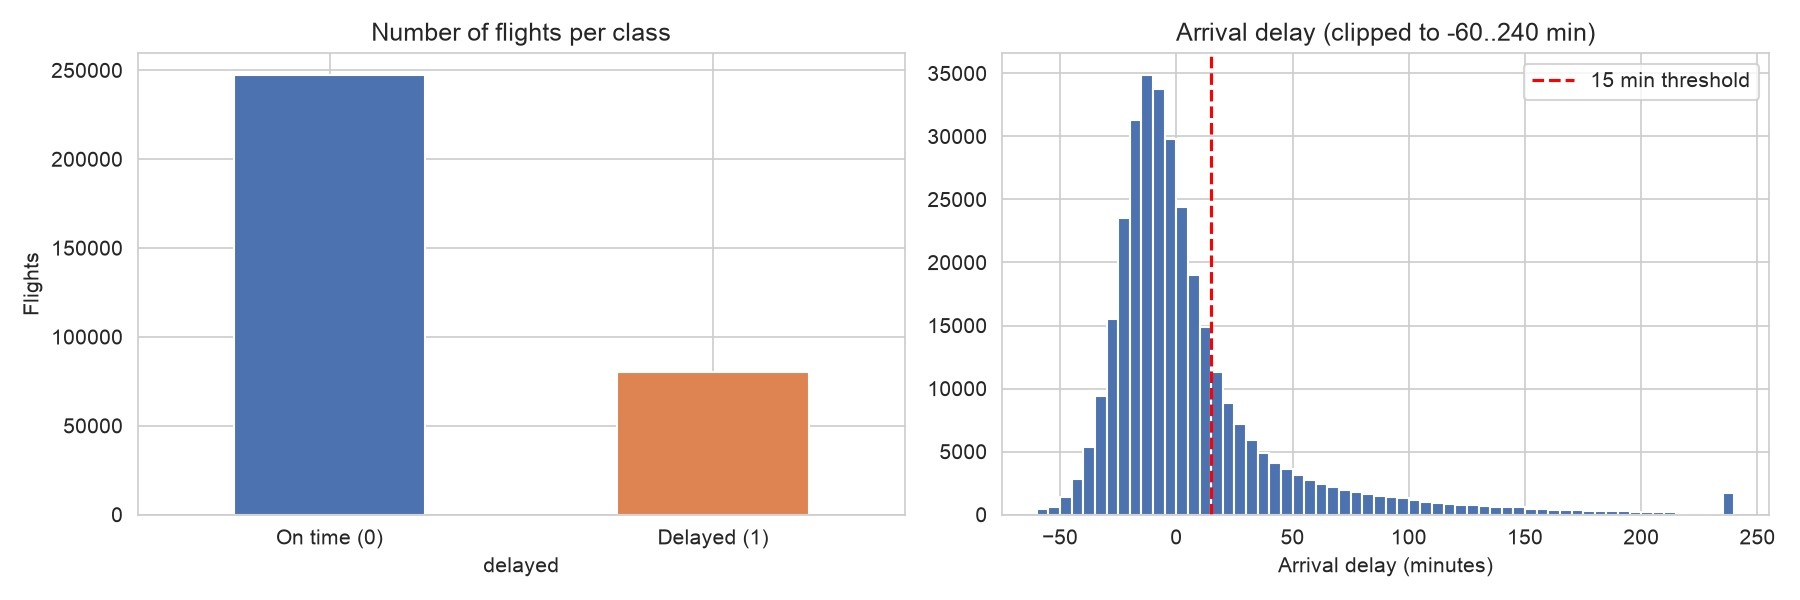
\includegraphics[width=\columnwidth]{target_distribution.png}
\caption{Class balance (left) and distribution of arrival delays (right).}
\label{fig:target}
\end{figure}

\subsection{Exploratory analysis}
Fig.~\ref{fig:time} shows the delay rate over time. December, July and June are the worst months (over 30\%
delayed) and September--November the calmest (under 20\%). Saturday has the lowest delay rate. The clearest
pattern is the hour of the day: about 10\% of 5~a.m.\ flights are delayed, rising to about 37\% at 9~p.m., as
delays build up through the network during the day. The delay rate also varies strongly by carrier, from 13\%
(HA) to 39\% (F9), and EWR is the most delayed of the three airports (26\%).

\begin{figure}[t]
\centering
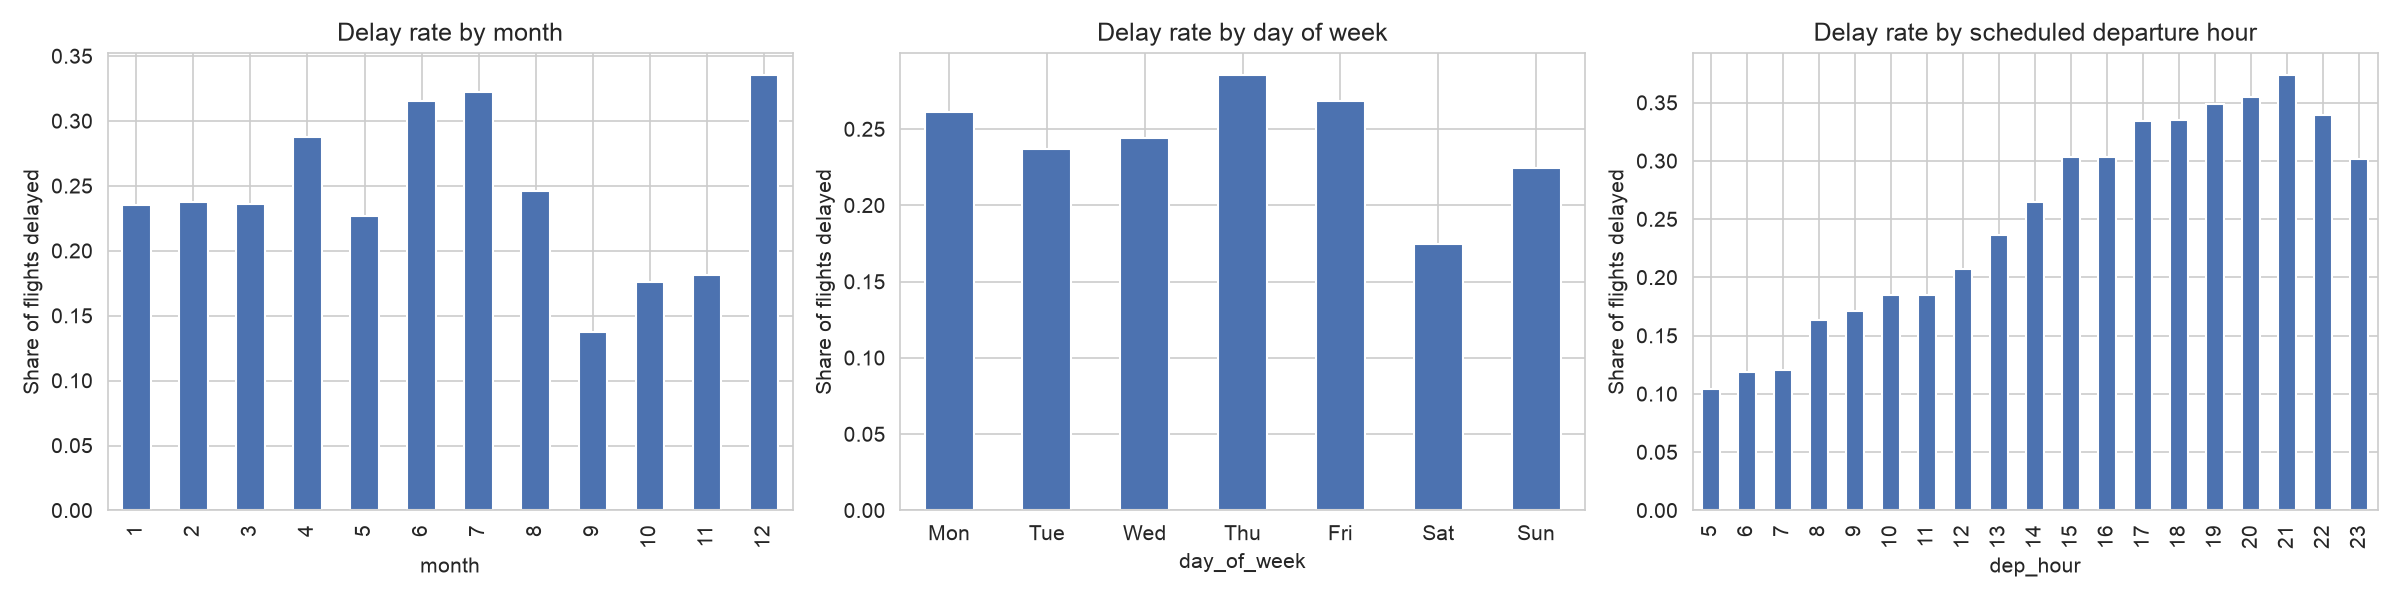
\includegraphics[width=\columnwidth]{delay_by_time.png}
\caption{Delay rate by month, day of week and scheduled departure hour.}
\label{fig:time}
\end{figure}

\section{Methodology}
\subsection{Preventing data leakage}
We assume the prediction is made before the flight departs, for example on the morning of the flight day. All
columns known only after departure are removed: actual departure and arrival times, departure and arrival delay
(the arrival delay is used only to build the target) and air time. We also drop the tail number (aircraft can be
swapped and it has about 4{,}000 values), the flight number and redundant date/time columns.

\subsection{Features}
\begin{itemize}
\item \textbf{Calendar/schedule:} weekend flag, distance, and the day of week and scheduled departure and arrival
hour with \emph{cyclic encoding}: each value $t$ with period $P$ ($P=24$ for hours, $P=7$ for days) becomes
$\sin(2\pi t/P)$ and $\cos(2\pi t/P)$, so that hour 23 is close to hour 0 and Sunday is close to Monday.
\item \textbf{Categorical:} carrier, origin and destination (one-hot encoded).
\item \textbf{Congestion:} number of flights scheduled to leave the same airport in the same hour and on the same day.
These counts use the full schedule, including flights that were later cancelled: counting only completed flights
would leak information, since bad-weather days have many cancellations.
\item \textbf{Route and history:} the route is the origin--destination pair (223 routes, e.g.\ JFK--LAX). For
the carrier, origin, destination and route we compute the share of delayed flights over the previous seven
calendar days. Daily counts of delayed and total flights are summed over a 7-day window that is shifted by
one day, so a flight never sees its own day or the future. Missing values (no history yet) are filled with the training mean.
\end{itemize}
The month is not used as a feature because the test months never appear in the training data.

\subsection{Data split}
The data are split by date: train January--August (217{,}727 flights, 26.4\% delayed), validation
September--October (55{,}628, 15.7\%) and test November--December (53{,}991, 25.8\%). The test set is used once.

\subsection{Models}
\textbf{Logistic Regression} models $P(y=1\mid x)=\sigma(w^\top x+b)$ and minimises the L2-regularised log loss.
Features are standardised and the classes are weighted inversely to their frequency.

\textbf{XGBoost} builds an ensemble $\hat y(x)=\sum_k f_k(x)$ of regression trees. Each
new tree minimises a second-order approximation of the loss plus a penalty
$\Omega(f)=\gamma T+\frac{1}{2}\lambda\lVert w\rVert^2$ on the number of leaves $T$ and leaf weights $w$. We use
learning rate 0.05, row and column subsampling of 0.8, minimum child weight 50, and
\texttt{scale\_pos\_weight} equal to the ratio of negative to positive training examples.

\textbf{Tuning.} Because delay patterns change with the season, a single validation period is a noisy guide. We
therefore use expanding-window time-series validation with three folds (train Jan--Apr/validate May--Jun,
Jan--Jun/Jul--Aug, Jan--Aug/Sep--Oct) and choose the tree depth $\in\{3,4,6\}$ and number of trees
$\in\{100,300\}$ with the best mean PR AUC. The best setting was depth 3 with 100 trees (mean PR AUC 0.377); larger models did worse
on future months. The final model is trained on the training set.

\subsection{Evaluation and calibration}
We report PR AUC (average precision), ROC AUC, recall at precision $\ge 0.5$ (the highest recall on the test
precision--recall curve where precision is at least 0.5) and the Brier score
$\frac{1}{N}\sum_i (p_i-y_i)^2$. Class weighting makes the raw probabilities too high, so we fit an isotonic
regression from model scores to outcomes on the validation set and apply it to the test set.

\section{Results}
Table~\ref{tab:results} and Fig.~\ref{fig:curves} summarise the test results. Both models are clearly better than
random. XGBoost has the best PR AUC and ROC AUC, and its advantage is largest at high precision: when 50\% of
alerts must be real delays, it finds 11.1\% of all delayed flights compared with 5.9\% for Logistic Regression.

\begin{table}[t]
\centering
\caption{Test set results (November--December 2013)}
\label{tab:results}
\setlength{\tabcolsep}{4pt}
\begin{tabular}{lcccc}
\toprule
Model & PR AUC & ROC AUC & Rec@P0.5 & Brier \\
\midrule
Random guess & 0.258 & 0.500 & -- & -- \\
Log. Regression & 0.376 & 0.645 & 0.059 & 0.228 \\
XGBoost & \textbf{0.391} & \textbf{0.656} & \textbf{0.111} & \textbf{0.219} \\
\bottomrule
\end{tabular}
\end{table}

\begin{figure}[t]
\centering
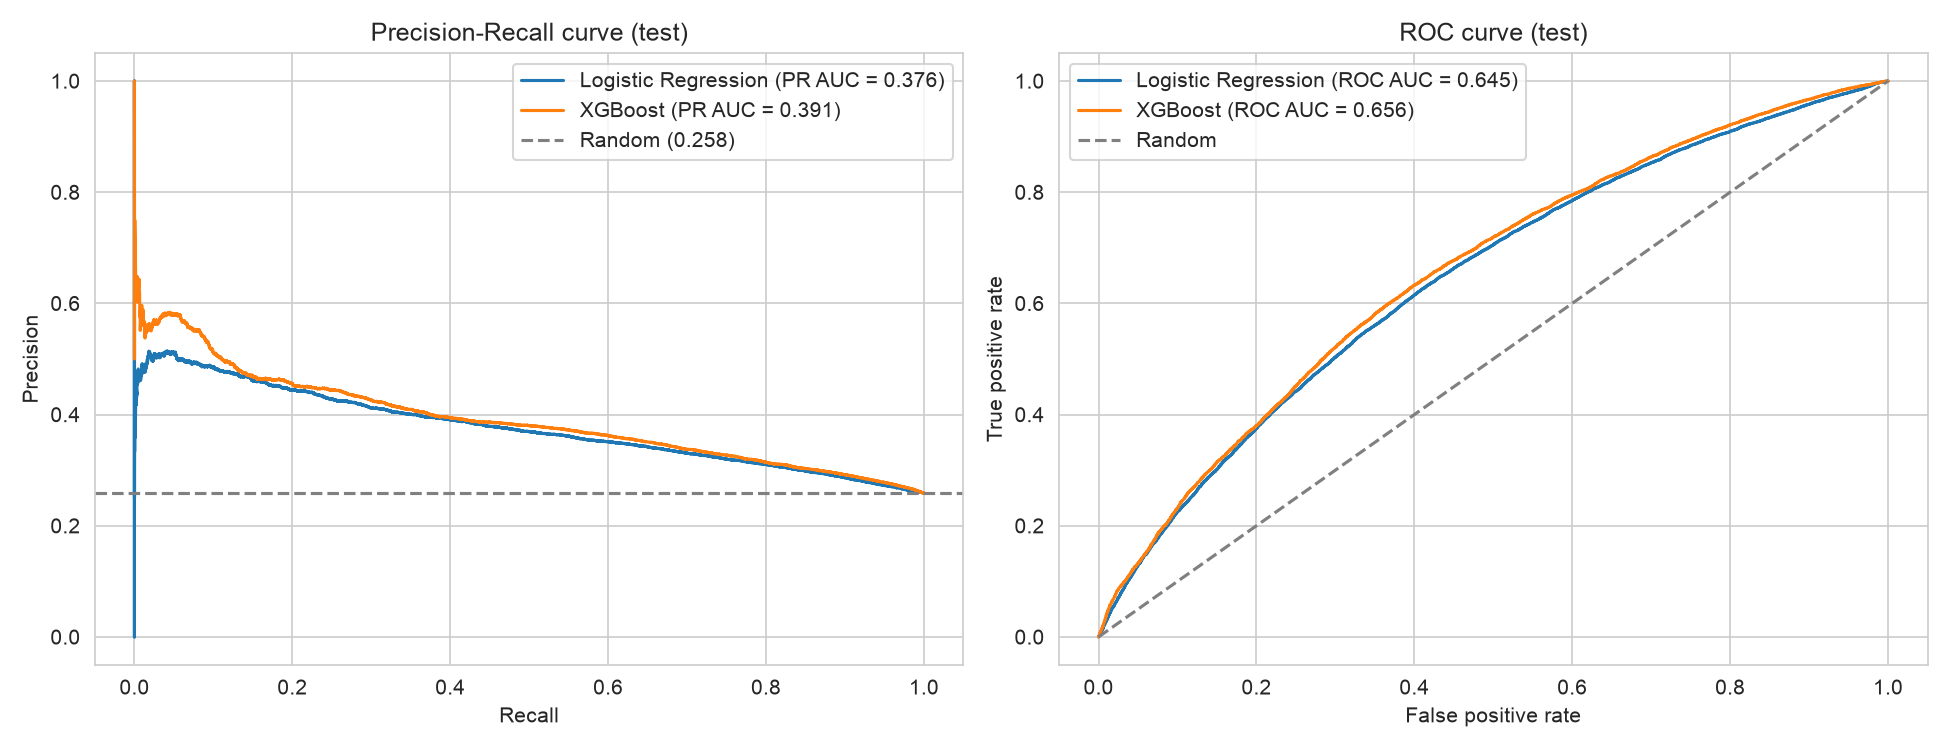
\includegraphics[width=\columnwidth]{pr_roc_curves.png}
\caption{Precision--recall and ROC curves on the test set.}
\label{fig:curves}
\end{figure}

\textbf{Calibration.} Before calibration both models over-estimate the delay probability (Fig.~\ref{fig:calib}).
After isotonic calibration the Brier score falls to 0.190 (Logistic Regression) and 0.188 (XGBoost). The
calibrated models under-estimate delays because the calibration months were calmer than the test months.
A constant prediction of the test delay rate would score 0.192, so the calibrated probabilities are reliable but
only somewhat sharper than the average.

\begin{figure}[t]
\centering
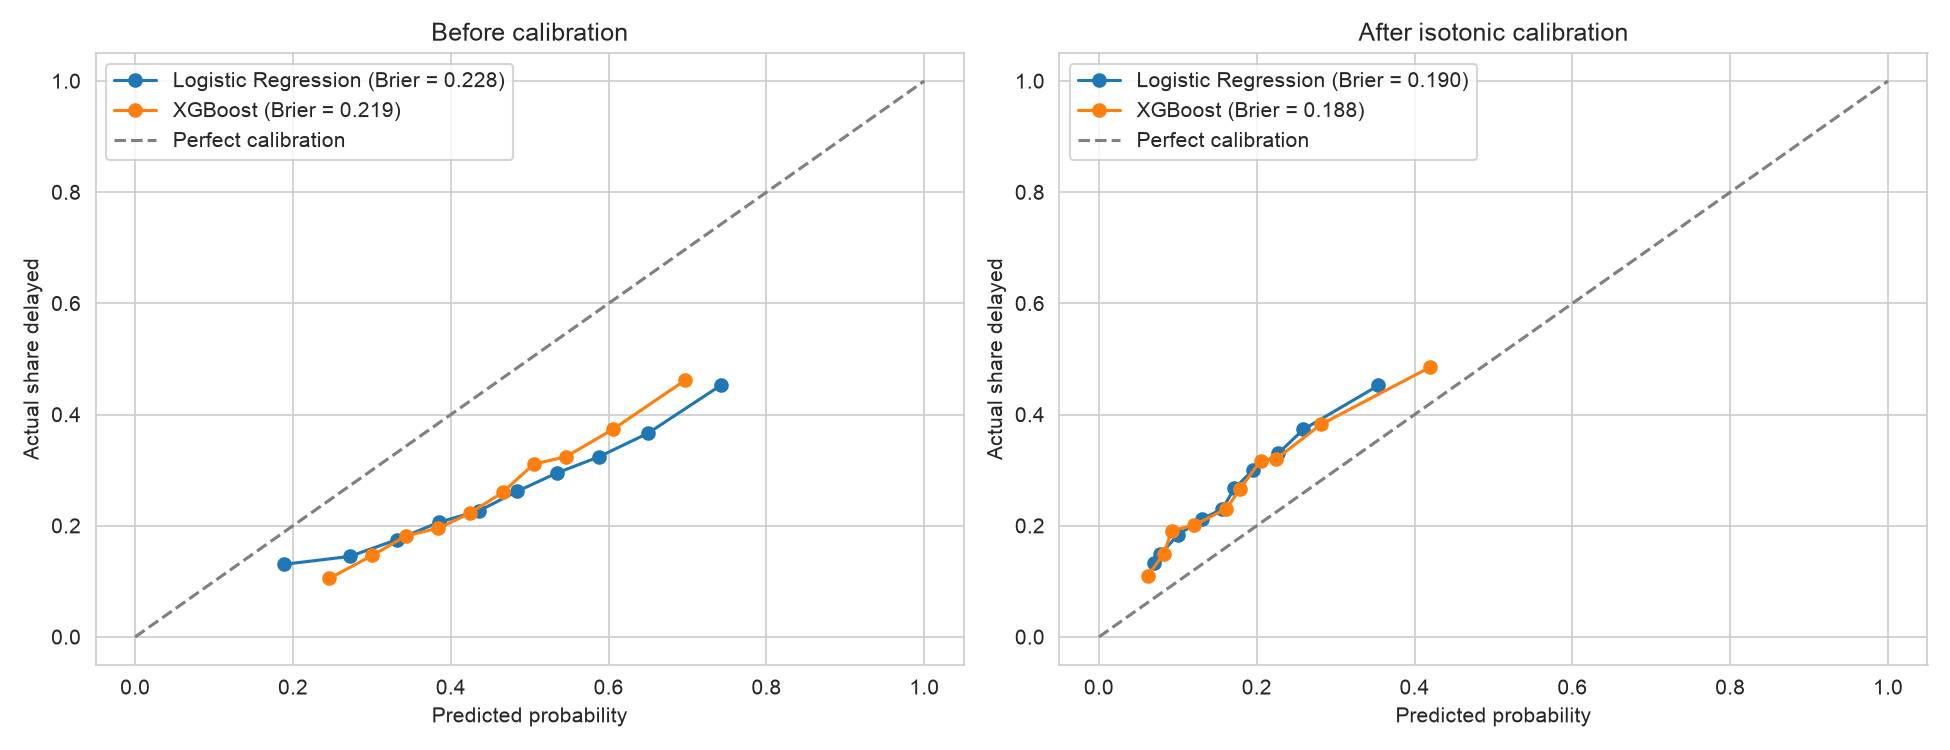
\includegraphics[width=\columnwidth]{calibration.png}
\caption{Reliability diagrams on the test set before and after isotonic calibration.}
\label{fig:calib}
\end{figure}

\textbf{Feature importance.} The cyclic encodings of the scheduled departure and arrival hours are the most
important XGBoost features, followed by the carrier's recent delay rate, the number of flights scheduled from the
origin that day, the route's recent delay rate and specific carriers (e.g.\ EV) (Fig.~\ref{fig:importance}). The
largest standardised Logistic Regression coefficients agree: the sine of the departure hour has a large negative
weight (it is negative for afternoon and evening hours, so later flights get a higher risk), while daily scheduled
flights at the origin and the recent delay rates of the route and carrier have positive weights. In short, later,
busier and recently delayed flights are more often late.

\begin{figure}[t]
\centering
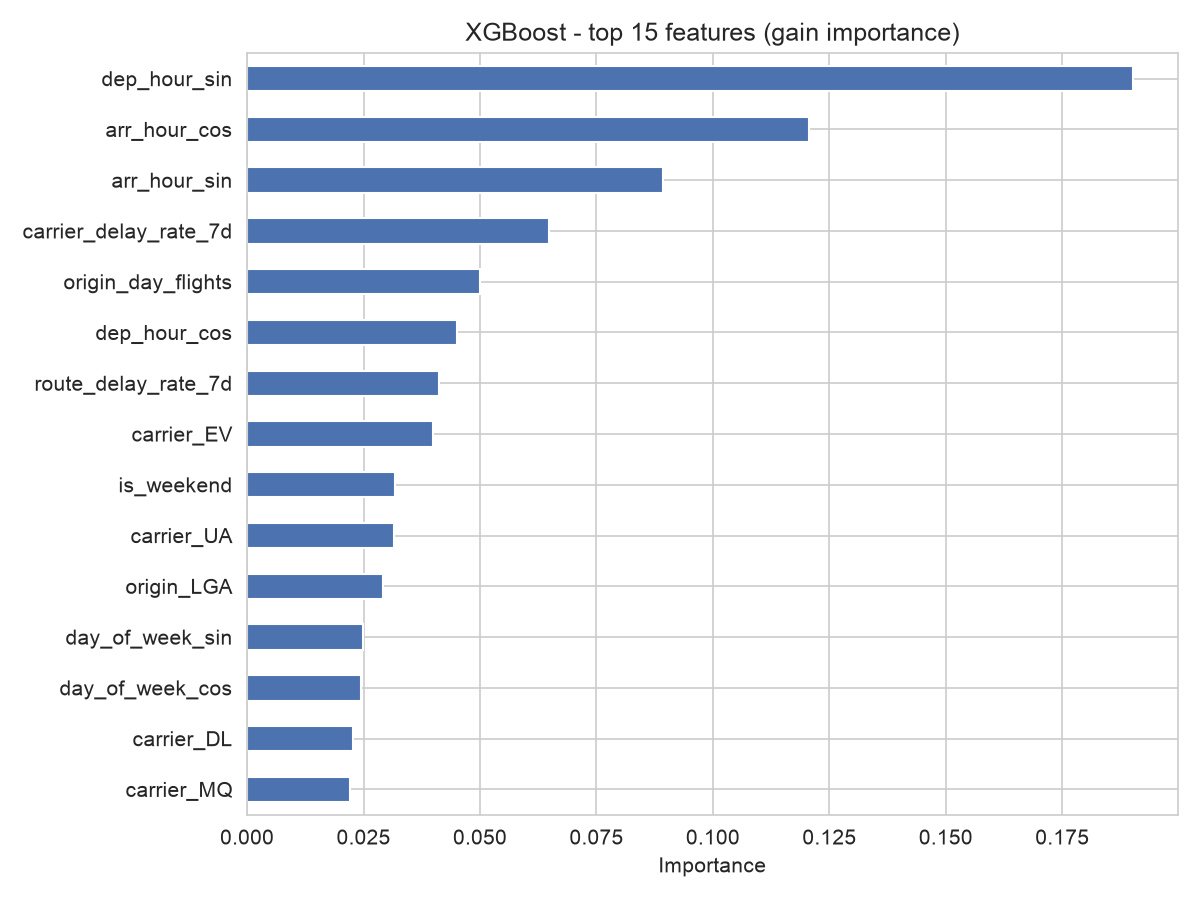
\includegraphics[width=0.9\columnwidth]{feature_importance.png}
\caption{Top 15 XGBoost features by gain.}
\label{fig:importance}
\end{figure}

\section{Discussion and Limitations}
Predicting delays before departure is hard: most delays are caused by weather, air traffic control and
knock-on effects from earlier flights, none of which are fully known in advance. An ROC AUC around 0.65 is
therefore expected for schedule-based features. Other limitations are that the data cover only New York
airports in 2013; that the test period (November--December) differs from the training months, which affects
both tuning and calibration; and that no weather data were used.

\section{Conclusion and Future Work}
Using only pre-departure information and a strict date-based evaluation, XGBoost predicts arrival delays better
than Logistic Regression, especially at high precision, and isotonic calibration gives reliable probabilities.
The time of day and the recent delay history of the carrier are the strongest signals. In Phase 2 we will train
a neural network with learned embeddings for carriers, origins and destinations and compare it with these
baselines under the same split and metrics. Adding forecast weather at the origin airport is another natural
extension.

\end{document}
